\documentclass[11pt]{article}
\usepackage[margin=1in]{geometry}
\usepackage{amsmath,booktabs,graphicx,float}
\title{CGMYW Lévy Model: P-then-Q Calibration on AAPL\\\large Progress Report}
\author{Vishwak Velamuri}
\date{November 2, 2026}
\begin{document}
\maketitle

\section{Summary}
I built and tested the full two-stage pipeline for the 8-parameter asymmetric CGMYW model
$(C_n,C_p,G,M,Y_n,Y_p,W_n,W_p)$, using AAPL:
\begin{enumerate}
\item \textbf{P-measure:} fit to daily CRSP returns over a trailing 252-trading-day window by
Anderson--Darling-weighted tail-probability matching (30 thresholds spanning the distribution, 8-start optimizer).
\item \textbf{Q-measure:} Carr--Madan FFT pricer; calibrate to a 30--45 day OTM option smile using a
vega-weighted price error. $M$ is solved from the martingale condition
$T\,\psi_Q(-i)=\ln(F/S_0)$, so every candidate is a martingale measure. Main fit
(per our 2026-10-19 discussion): $C_n,C_p,G,W_n,W_p$ free, $Y_n,Y_p$ pinned at P values.
\end{enumerate}
\textbf{Headline:} the main Q fit matches the market smile to \textbf{0.97} and \textbf{0.74} implied-vol
points on the two test dates. The automated test suite passes in full (\textbf{138/138 tests}).

\textbf{New (2026-11-02):} a 9-parameter Sato CGMYW fit to four maturities at once (1 month to 1 year) has a median
error of \textbf{0.99 vol points} over 18 dates and beats the Lévy model on every date; $W$ adds little to the surface fit (Section~6).

\section{Correctness checks}
Each piece is checked against an independent reference before any market data is used.
\begin{table}[H]\centering\small
\begin{tabular}{p{6.2cm}p{4.2cm}l}\toprule
Check & Reference & Result\\\midrule
Closed form with $W_n=W_p=0$, $C_n=C_p$, $Y_n=Y_p$ & classical CGMY $\psi$ & error $<10^{-8}$ over $|u|\le300$\\
Power-tilt term ($W\neq0$) & direct 30-digit quadrature of $\int(e^{iux}-1)k(x)dx$ & rel.\ error $\sim10^{-14}$\\
Kummer $U$ for complex $z$ & mpmath & passes (both branches)\\
Lévy density $\to$ PDF normalization & integrates to 1 & passes\\
Carr--Madan FFT & Black--Scholes closed form & error $<10^{-5}$ (Fig.~\ref{fig:checks})\\
CGMYW option prices & Gil--Pelaez quadrature & error $<10^{-4}$\\
Risk-neutralization & Madan--Wang Table 2, all 10 tickers & $G,M$ within 0.2\%; $W$ within 0.22\\
Synthetic smile & known Q parameters & recovered, IV RMSE $<0.2$ vol pts\\\bottomrule
\end{tabular}\end{table}
On the Table 2 reproduction: started from the paper's own values or from the P values, our minimum-norm
solve lands on the same point. That point meets the martingale condition to $10^{-12}$; the published
values meet it only to about $10^{-5}$. The small gap in $W$ therefore comes from the paper's solver
tolerance, not from a model error.

\begin{figure}[H]\centering
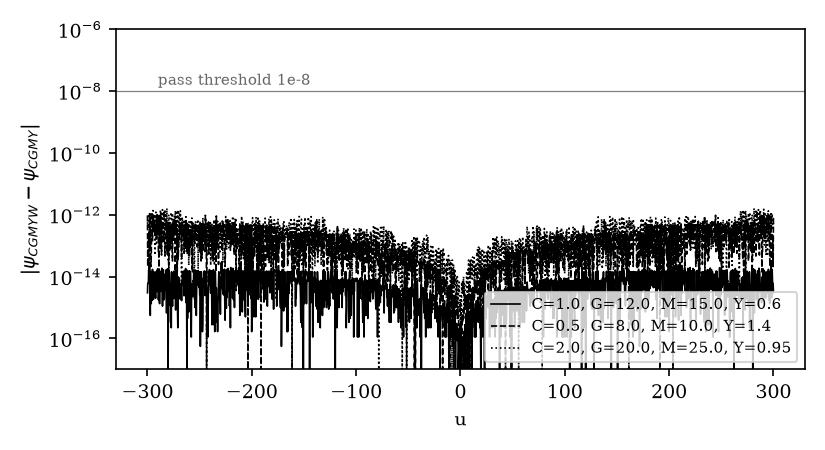
\includegraphics[width=.49\textwidth]{figures/check_reduction.png}
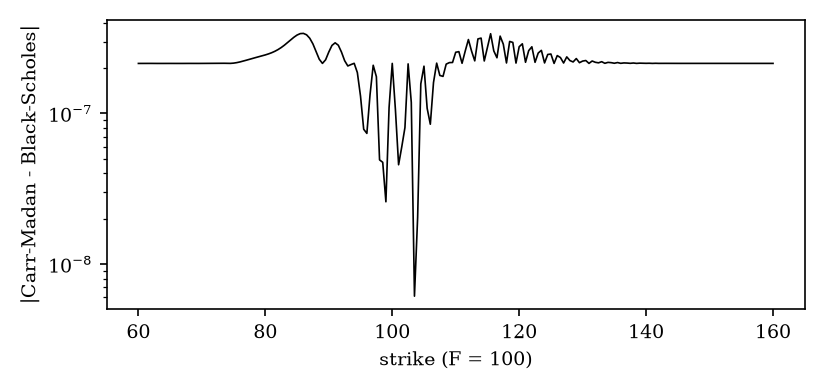
\includegraphics[width=.49\textwidth]{figures/check_carr_madan.png}
\caption{Left: CGMYW reduces to classical CGMY (error at machine precision). Right: FFT pricer vs.\ Black--Scholes.}
\label{fig:checks}\end{figure}

\section{P-measure results (AAPL)}
\begin{table}[H]\centering\small
\begin{tabular}{lrrrrrrrrr}\toprule
Window end & $C_n$ & $C_p$ & $G$ & $M$ & $Y_n$ & $Y_p$ & $W_n$ & $W_p$ & AD obj.\\\midrule
2023-01-13 & 3.803 & 3.920 & 118.2 & 143.9 & 0.053 & 0.061 & 14.86 & 4.83 & 0.0151\\
2025-08-29 & 0.543 & 0.888 & 41.0 & 94.5 & 0.043 & 0.051 & 14.57 & 5.03 & 0.0206\\\midrule
Madan--Wang T1 & 0.952 & 1.344 & 52.0 & 97.6 & 0.003 & 0.003 & 22.27 & 4.83 & --\\\bottomrule
\end{tabular}
\caption{Daily units; 251 returns per window; all 8 optimizer starts converged on both dates.
The paper uses a fixed 1033-day window, but our fits land in the same regime: small $Y$, $W_n\gg W_p$, $M>G$.}
\end{table}
\begin{figure}[H]\centering
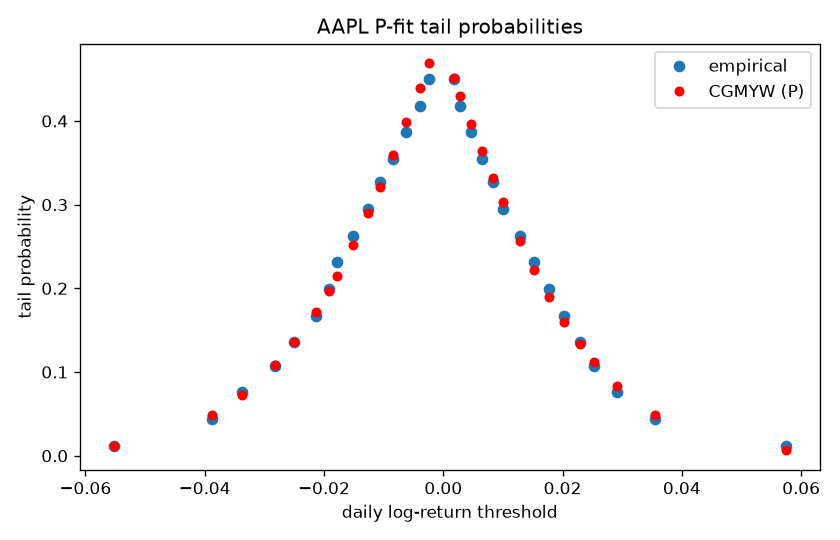
\includegraphics[width=.49\textwidth]{figures/aapl_20230113_pfit_tails.png}
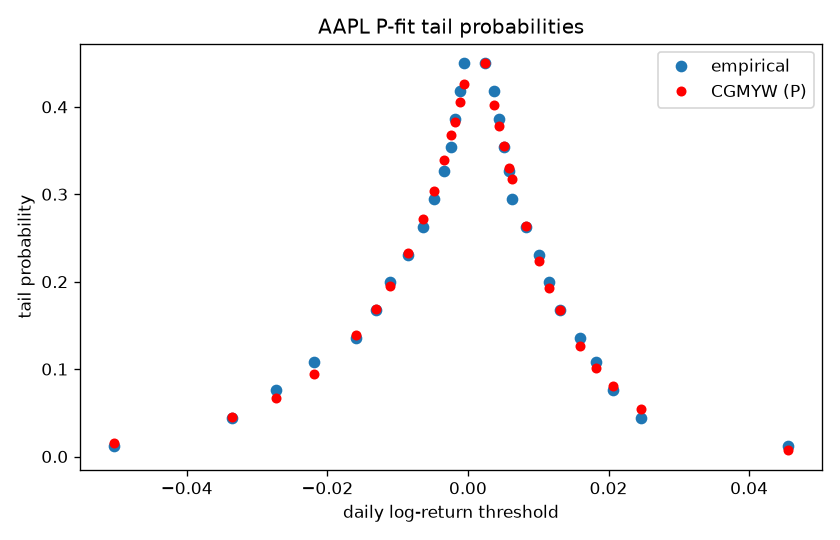
\includegraphics[width=.49\textwidth]{figures/aapl_20250829_pfit_tails.png}
\caption{Empirical vs.\ model tail probabilities. Left: 2023-01-13. Right: 2025-08-29.}
\end{figure}

\section{Q-measure results (AAPL)}
\begin{table}[H]\centering\small
\begin{tabular}{lcc}\toprule
IV RMSE (vol points) & 2023-01-13 $\to$ 02-24 (49 opts) & 2025-08-29 $\to$ 10-10 (24 opts)\\\midrule
P + martingale only (no option data) & 6.24 & 7.71\\
Strictly equivalent ($C,Y$ pinned) & 6.29 & 8.99\\
\textbf{Main: $C_n,C_p$ free, $Y$ pinned} & \textbf{0.97} & \textbf{0.74}\\
Unrestricted (all 8 free, diagnostic) & 0.42 & 0.14\\\bottomrule
\end{tabular}\end{table}
\begin{figure}[H]\centering
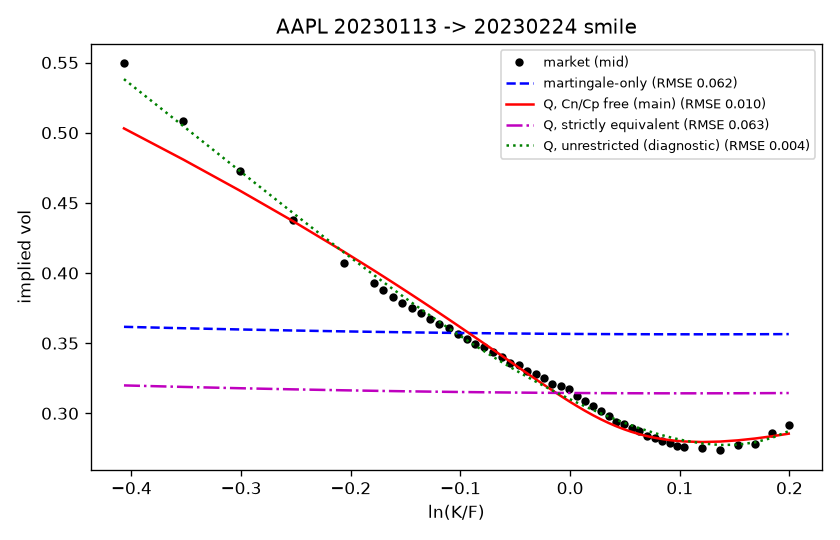
\includegraphics[width=.49\textwidth]{figures/aapl_20230113_smile.png}
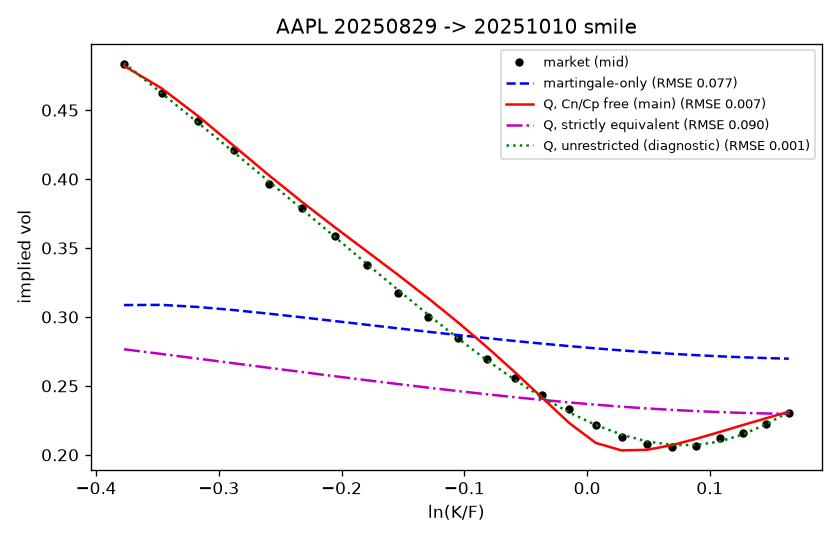
\includegraphics[width=.49\textwidth]{figures/aapl_20250829_smile.png}
\caption{Market vs.\ model implied-vol smiles, 42-day maturity.}
\end{figure}
\textbf{Main-fit parameters (annual):} 2023-01-13: $C_n=9.84, C_p=26.98, G=8.80, M=29.23, W_n=2.61, W_p=5.67$.
2025-08-29: $C_n=4.29, C_p=11.07, G=0.035, M=27.28, W_n=11.0, W_p\approx0$. On the second date the down tail
is carried almost entirely by the power tilt $W_n$, which is the role the model was designed for.

\section{Stability across 18 quote dates}
The full pipeline (fresh 252-day P-fit, then the main Q fit) was rerun on 18 quote dates, about every
two months from 2023-01 to 2025-08. Out of sample: the fitted Q parameters were used, without
refitting, to price a longer 60--120 day smile on the same date.
\begin{table}[H]\centering\small
\begin{tabular}{lccc}\toprule
& Median & Range & \\\midrule
Main Q fit, IV RMSE (vol pts) & 1.18 & 0.44--5.38 & under 2 on 14 of 18 dates\\
Out-of-sample maturity, IV RMSE (vol pts) & 2.83 & 0.76--6.54 & no refit\\
P tail-probability RMSE & 0.0107 & 0.0063--0.0164 & Madan--Wang AAPL: 0.0067 (1033 days)\\\bottomrule
\end{tabular}\end{table}
\begin{figure}[H]\centering
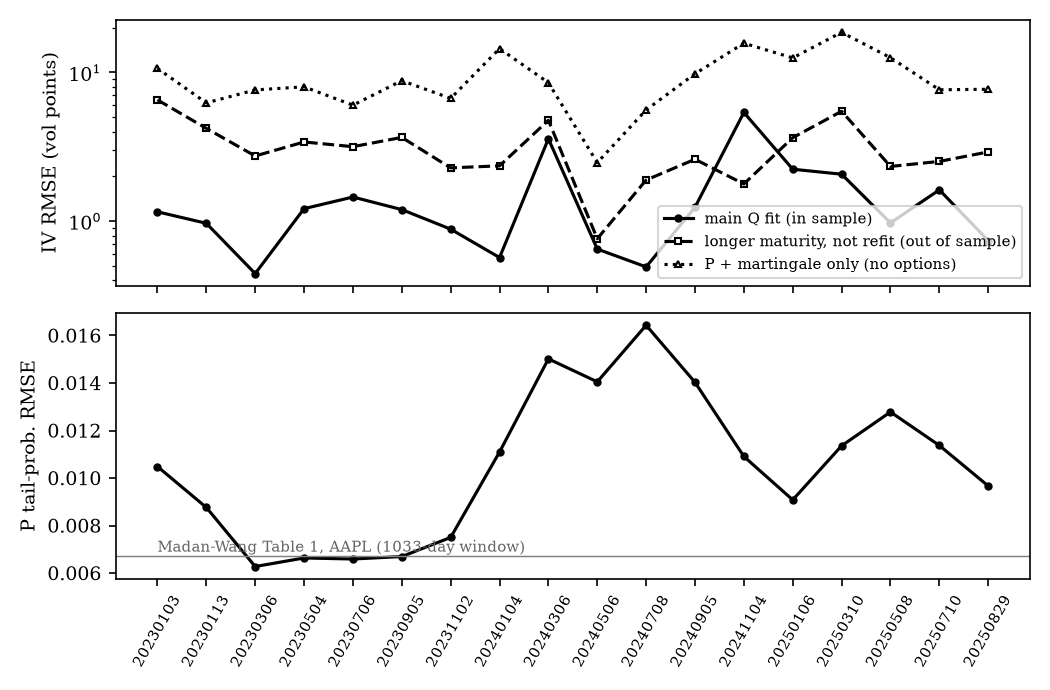
\includegraphics[width=.85\textwidth]{figures/stability.png}
\caption{Top: Q-fit error over time (log scale): in sample, out of sample, and P + martingale only.
Bottom: P-fit tail-probability RMSE per window.}
\end{figure}
The two weakest in-sample dates are 2024-11-04 (5.38) and 2024-03-06 (3.58). On every date, the option-free
martingale-only measure is far worse than the calibrated fit, so the option data is doing real work.
The out-of-sample error is roughly 2--3$\times$ the in-sample error: the parameters carry over across
maturities, but not perfectly.
\begin{figure}[H]\centering
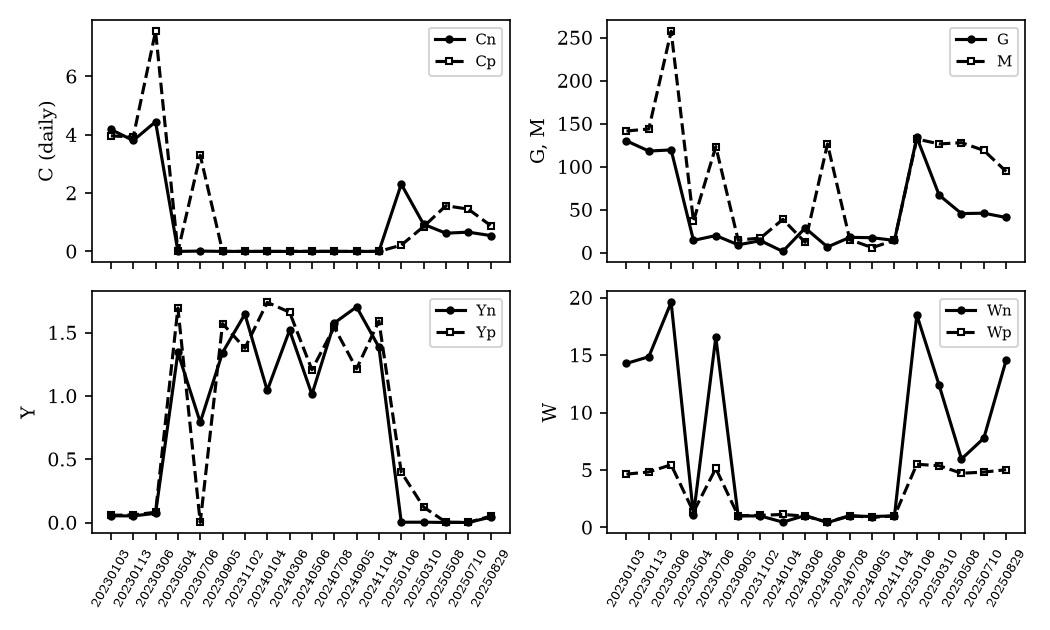
\includegraphics[width=.85\textwidth]{figures/p_params.png}
\caption{P-measure parameters across the 18 trailing windows.}
\end{figure}

\section{Option surface: Lévy vs.\ Sato, with and without $W$}
Following the 2026-11-02 meeting, a second calibration fits the whole option surface directly.
\begin{itemize}
\item \textbf{All parameters free.} The martingale condition is met by a constant,
$\ln S_T=\ln F+X_T+\omega_T$ with $\omega_T=-\ln E[e^{X_T}]$, instead of by solving for $M$.
\item \textbf{Forward from the options.} $F=S_0e^{(r-q)T}$, with $q$ implied so that $F$ is where call and put
mids cross (put-call parity). It lands within 0.5\% of WRDS's forward; implied $q\approx0.7$--$1.3\%$.
\item \textbf{Four maturities at once:} the traded expiries closest to 1, 3, 6 and 12 months, one parameter set.
\item \textbf{Sato process.} $X_T=T^\gamma X_1$ with $X_1$ CGMYW, so $E[e^{iuX_T}]=e^{\psi(uT^\gamma)}$: 9 parameters.
CGMYW is self-decomposable ($|x|k(x)$ decreasing in $|x|$ for $G,M,Y,W\ge0$), so this is a valid Sato process.
Under a Lévy process, skew decays like $T^{-1/2}$ and excess kurtosis like $T^{-1}$; under Sato both are flat in $T$.
\end{itemize}
Four models on the same 18 dates with the same objective: Lévy CGMY (6 parameters), Lévy CGMYW (8),
Sato CGMY (7), Sato CGMYW (9). Each CGMYW fit is warm-started from its CGMY fit, since it contains CGMY as the case $W=0$.
\begin{table}[H]\centering\small
\begin{tabular}{lcccccc}\toprule
& \multicolumn{2}{c}{Surface IV RMSE (vol pts)} & \multicolumn{4}{c}{Mean IV RMSE by maturity}\\
Model & median & range & $\sim$1m & $\sim$3m & $\sim$6m & $\sim$1y\\\midrule
Lévy CGMY  & 1.56 & 1.11--4.22 & 2.86 & 1.25 & 1.02 & 1.68\\
Lévy CGMYW & 1.52 & 1.07--4.22 & 2.81 & 1.21 & 1.01 & 1.63\\
Sato CGMY  & 1.00 & 0.43--1.52 & 1.86 & 1.00 & 0.47 & 0.89\\
\textbf{Sato CGMYW} & \textbf{0.99} & 0.43--1.52 & 1.85 & 0.98 & 0.45 & 0.88\\\bottomrule
\end{tabular}\end{table}
\begin{figure}[H]\centering
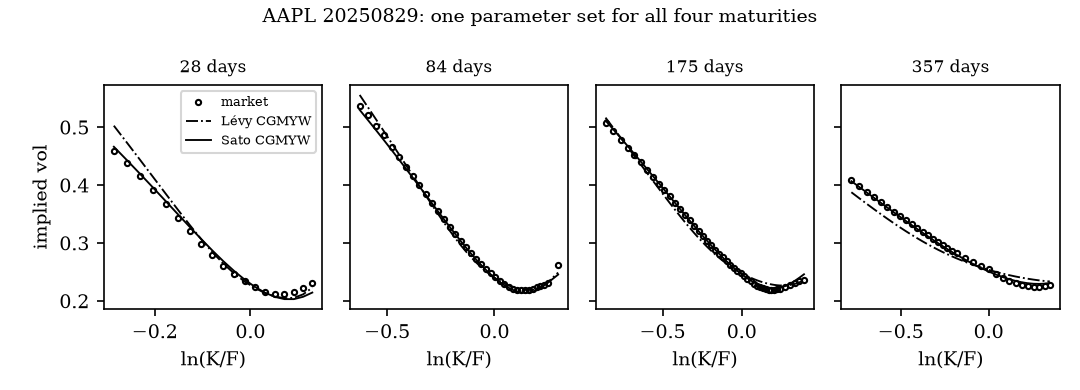
\includegraphics[width=\textwidth]{figures/surface_20250829.png}
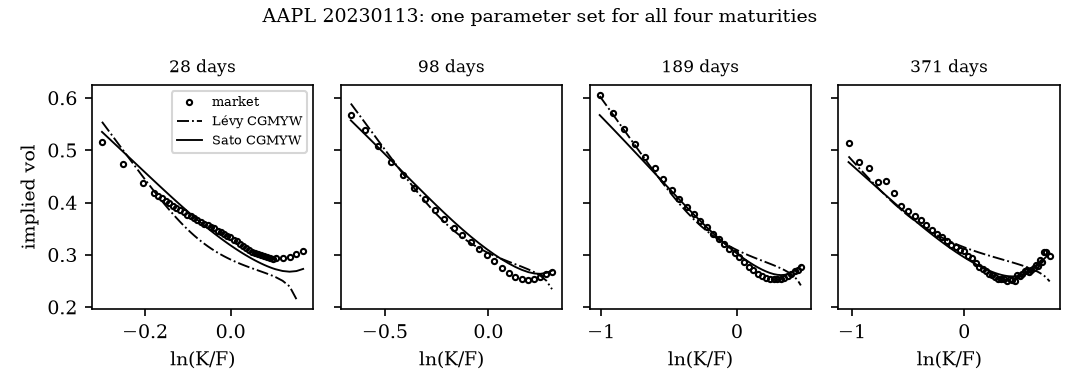
\includegraphics[width=\textwidth]{figures/surface_20230113.png}
\caption{One parameter set for four maturities. Lévy (dash-dot) is too steep at 1 month and too flat at 1 year;
Sato (solid) follows the term structure.}
\end{figure}
\begin{figure}[H]\centering
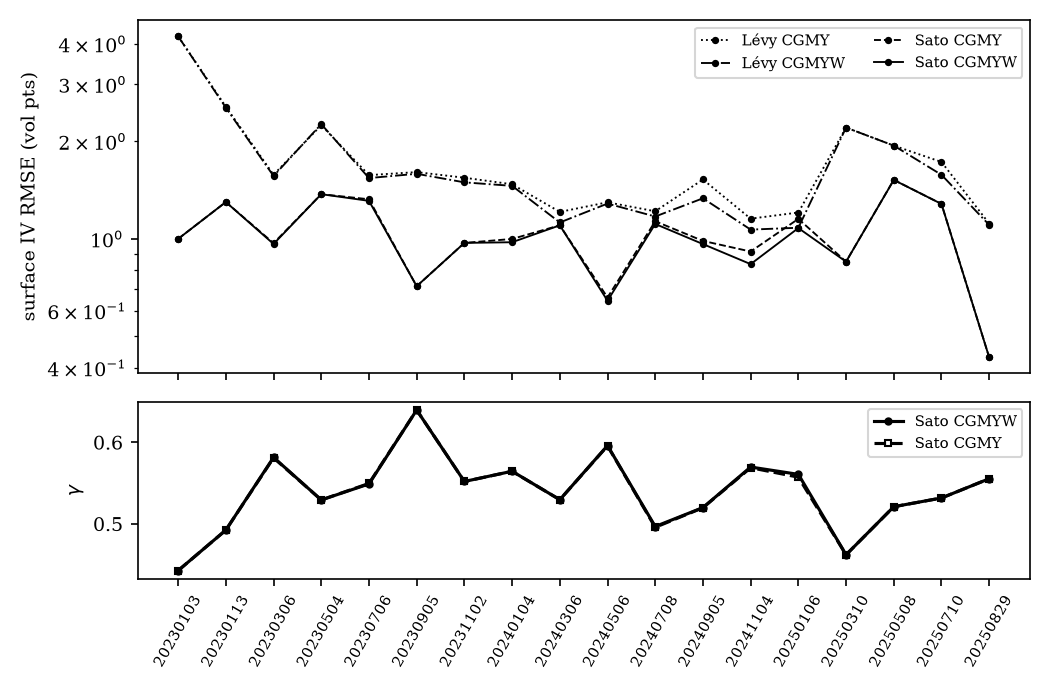
\includegraphics[width=.85\textwidth]{figures/surface_summary.png}
\caption{Top: surface IV RMSE per date for each model (log scale). Bottom: fitted $\gamma$.}
\end{figure}
\textbf{Results.}
\begin{itemize}
\item \textbf{Sato beats Lévy on all 18 dates}, with a median surface error of 1.0 vs.\ 1.5 vol points. Lévy fails
at the ends of the term structure (2.9 vol points at 1 month), as the $T^{-1/2}$, $T^{-1}$ argument predicts.
\item \textbf{$\gamma$ is stable:} median 0.54, range 0.44--0.64.
\item \textbf{$W$ adds little on the option surface.} Under Sato, the fit uses $W$ on only 6 of 18 dates
($W_n$ from 0.6 to 2.2, $W_p\approx0$ throughout), and the error falls by at most 8\% (2024-11-04: 0.91 $\to$ 0.84);
the median gain is 0. Under Lévy, $W$ lowers the fit objective on 15 of 18 dates; the IV error falls by a median 1.2\% and at most about 12\%
(2024-09-05: 1.52 $\to$ 1.33). Where $W$ is used, it is always on the down side, as in the P fits ($W_n\gg W_p$).
\item \textbf{Caveat:} $Y_p$ often sits at its lower bound and $Y_n\approx1.3$--$1.7$, which points to weak
identification of the up tail from four smiles. Nelder--Mead is a local method, but the nested consistency
(CGMYW never worse than CGMY) now holds on every date.
\end{itemize}

\section{Findings}
\begin{itemize}
\item The pricer and optimizer are not the bottleneck: the unrestricted fit reaches 0.14--0.42 vol points.
\item A strictly equivalent change of measure ($C,Y$ fixed) cannot produce AAPL's put skew (6--9 vol pts).
With no diffusion term, the martingale condition forces the two tails to nearly cancel.
\item Freeing $C_n,C_p$ (as in the Markovian-economies paper) closes most of the gap: under 1 vol point.
Risk-neutral $C$ comes out below physical $C$ on both sides.
\item $(C,Y)$ are only weakly identified from 251 daily returns, and those are exactly the parameters pinned in Q.
\item Across maturities, the time dimension matters far more than $W$: Sato vs.\ Lévy is worth about 0.5 vol points;
$W$ is worth about 0.02 under Sato.
\end{itemize}

\section{Next steps}
Run the Lévy/Sato, $W$/no-$W$ comparison on all 10 stocks (no stock-specific code paths exist); check whether
$W$ matters more for names with heavier down tails; tighten identification of the up tail ($Y_p$ at its bound);
build the estimation notebook.
\end{document}
